\documentclass[../main.tex]{subfiles}

\title{Linear Algebra}
\author{}
\date{}

\begin{document}

\maketitle
\tableofcontents

\newpage

\section{Vectors}

\subsection{Geometry}

A vector in 2 dimensional space is an oriented length.
In 3 dimensions, vectors are oriented ares.
Then oriented volumes, and so on.
They can represent a position in space, or a displacement (change in position).

\subsection{Coordinates}

Numerically, vectors describe things along different dimensions or aspects.
We do this by fixing an origin and a basis.
Each axis represents a dimension we want to talk about,
and the origin represents 0.
Then a length along each axis represents a quantity along each dimension.

In Euclidean space, it is convenient to use the standard basis.
To identify each oriented length with coordinates,
we put the tail at the origin and describe the length along each axis where the head is.
These are the coordinates of the vector relative to a given basis.
Thus,
any vector \( v \) is just the linear combination of its coordinates
with the corresponding basis vectors
\( v_1 e_1 + \dots + v_n e_n \).

\noindent
\begin{tikzpicture}[x=0.75pt,y=0.75pt,yscale=-1,xscale=1]
%uncomment if require: \path (0,300); %set diagram left start at 0, and has height of 300

%Shape: Circle [id:dp6722596476060768] 
\draw   (103,86.25) .. controls (103,78.93) and (108.93,73) .. (116.25,73) .. controls (123.57,73) and (129.5,78.93) .. (129.5,86.25) .. controls (129.5,93.57) and (123.57,99.5) .. (116.25,99.5) .. controls (108.93,99.5) and (103,93.57) .. (103,86.25) -- cycle ;
%Shape: Circle [id:dp74444730195737] 
\draw   (140,86.25) .. controls (140,78.93) and (145.93,73) .. (153.25,73) .. controls (160.57,73) and (166.5,78.93) .. (166.5,86.25) .. controls (166.5,93.57) and (160.57,99.5) .. (153.25,99.5) .. controls (145.93,99.5) and (140,93.57) .. (140,86.25) -- cycle ;
%Shape: Circle [id:dp9832620880412448] 
\draw   (230,86.25) .. controls (230,78.93) and (235.93,73) .. (243.25,73) .. controls (250.57,73) and (256.5,78.93) .. (256.5,86.25) .. controls (256.5,93.57) and (250.57,99.5) .. (243.25,99.5) .. controls (235.93,99.5) and (230,93.57) .. (230,86.25) -- cycle ;
%Shape: Brace [id:dp5022040197364186] 
\draw   (236.5,57) .. controls (236.5,52.33) and (234.17,50) .. (229.5,50) -- (188,50) .. controls (181.33,50) and (178,47.67) .. (178,43) .. controls (178,47.67) and (174.67,50) .. (168,50)(171,50) -- (126.5,50) .. controls (121.83,50) and (119.5,52.33) .. (119.5,57) ;
%Shape: Square [id:dp23486906391618334] 
\draw   (100,171) -- (126.5,171) -- (126.5,197.5) -- (100,197.5) -- cycle ;
%Shape: Square [id:dp8514361205022334] 
\draw   (134,171) -- (160.5,171) -- (160.5,197.5) -- (134,197.5) -- cycle ;
%Shape: Square [id:dp5165693986546934] 
\draw   (226,172) -- (252.5,172) -- (252.5,198.5) -- (226,198.5) -- cycle ;
%Shape: Brace [id:dp2319346457546657] 
\draw   (110.5,221) .. controls (110.5,225.67) and (112.83,228) .. (117.5,228) -- (169,228) .. controls (175.67,228) and (179,230.33) .. (179,235) .. controls (179,230.33) and (182.33,228) .. (189,228)(186,228) -- (240.5,228) .. controls (245.17,228) and (247.5,225.67) .. (247.5,221) ;
%Straight Lines [id:da9665534418589774] 
\draw    (113.25,170) -- (113.25,131) ;
\draw [shift={(113.25,129)}, rotate = 450] [color={rgb, 255:red, 0; green, 0; blue, 0 }  ][line width=0.75]    (10.93,-3.29) .. controls (6.95,-1.4) and (3.31,-0.3) .. (0,0) .. controls (3.31,0.3) and (6.95,1.4) .. (10.93,3.29)   ;
%Straight Lines [id:da2232187544111287] 
\draw    (148.25,171) -- (148.25,132) ;
\draw [shift={(148.25,130)}, rotate = 450] [color={rgb, 255:red, 0; green, 0; blue, 0 }  ][line width=0.75]    (10.93,-3.29) .. controls (6.95,-1.4) and (3.31,-0.3) .. (0,0) .. controls (3.31,0.3) and (6.95,1.4) .. (10.93,3.29)   ;
%Straight Lines [id:da8929455340252761] 
\draw    (240.25,169) -- (240.25,130) ;
\draw [shift={(240.25,128)}, rotate = 450] [color={rgb, 255:red, 0; green, 0; blue, 0 }  ][line width=0.75]    (10.93,-3.29) .. controls (6.95,-1.4) and (3.31,-0.3) .. (0,0) .. controls (3.31,0.3) and (6.95,1.4) .. (10.93,3.29)   ;

% Text Node
\draw (185,86.4) node [anchor=north west][inner sep=0.75pt]    {$\dotsc $};
% Text Node
\draw (170,14.4) node [anchor=north west][inner sep=0.75pt]    {$n$};
% Text Node
\draw (180,187.4) node [anchor=north west][inner sep=0.75pt]    {$\dotsc $};
% Text Node
\draw (175,248.4) node [anchor=north west][inner sep=0.75pt]    {$r$};


\end{tikzpicture}


\subsection{Addition and subtraction}

Adding a vector to another is simply just adding the quantities along each dimension.
Subtraction is taking the difference.

Geometrically, we can add two vectors \( \vb{u} \) and \( \vb{v} \)
by considering where we end up if we start at position \( \vb{u} \)
then apply the change \( \va{v} \).
Thus, \( \vb{u} + \va{v} = \vb{z} \).

\noindent
\tikzset{every picture/.style={line width=0.75pt}} %set default line width to 0.75pt        

\begin{tikzpicture}[x=0.75pt,y=0.75pt,yscale=-1,xscale=1]
%uncomment if require: \path (0,300); %set diagram left start at 0, and has height of 300

%Shape: Axis 2D [id:dp7522167816409159] 
\draw  (50,242) -- (419.5,242)(97.5,8) -- (97.5,267) (412.5,237) -- (419.5,242) -- (412.5,247) (92.5,15) -- (97.5,8) -- (102.5,15) (146.5,237) -- (146.5,247)(195.5,237) -- (195.5,247)(244.5,237) -- (244.5,247)(293.5,237) -- (293.5,247)(342.5,237) -- (342.5,247)(391.5,237) -- (391.5,247)(92.5,193) -- (102.5,193)(92.5,144) -- (102.5,144)(92.5,95) -- (102.5,95)(92.5,46) -- (102.5,46) ;
\draw   ;
%Shape: Circle [id:dp1800333897763694] 
\draw   (297,120.75) .. controls (297,117.57) and (299.57,115) .. (302.75,115) .. controls (305.93,115) and (308.5,117.57) .. (308.5,120.75) .. controls (308.5,123.93) and (305.93,126.5) .. (302.75,126.5) .. controls (299.57,126.5) and (297,123.93) .. (297,120.75) -- cycle ;
%Curve Lines [id:da6744184215507455] 
\draw    (98,171) .. controls (107.79,163.66) and (111.03,107.89) .. (139.27,154.95) .. controls (167.5,202) and (206.02,160.39) .. (242.5,187) .. controls (278.98,213.61) and (267.5,117) .. (297,120.75) ;
%Straight Lines [id:da042236632067626734] 
\draw [color={rgb, 255:red, 255; green, 0; blue, 0 }  ,draw opacity=1 ]   (302,103) -- (302,62) ;
\draw [shift={(302,60)}, rotate = 450] [color={rgb, 255:red, 255; green, 0; blue, 0 }  ,draw opacity=1 ][line width=0.75]    (10.93,-3.29) .. controls (6.95,-1.4) and (3.31,-0.3) .. (0,0) .. controls (3.31,0.3) and (6.95,1.4) .. (10.93,3.29)   ;
%Straight Lines [id:da8879089279998805] 
\draw [color={rgb, 255:red, 255; green, 0; blue, 0 }  ,draw opacity=1 ]   (301.75,136.5) -- (301.75,175) ;
\draw [shift={(301.75,177)}, rotate = 270] [color={rgb, 255:red, 255; green, 0; blue, 0 }  ,draw opacity=1 ][line width=0.75]    (10.93,-3.29) .. controls (6.95,-1.4) and (3.31,-0.3) .. (0,0) .. controls (3.31,0.3) and (6.95,1.4) .. (10.93,3.29)   ;
%Straight Lines [id:da984234265425485] 
\draw  [dash pattern={on 0.84pt off 2.51pt}]  (302.75,126.5) -- (302.75,245) ;
%Straight Lines [id:da851126430686476] 
\draw [color={rgb, 255:red, 0; green, 42; blue, 255 }  ,draw opacity=1 ]   (267,260) -- (298.5,260) ;
\draw [shift={(300.5,260)}, rotate = 180] [color={rgb, 255:red, 0; green, 42; blue, 255 }  ,draw opacity=1 ][line width=0.75]    (10.93,-3.29) .. controls (6.95,-1.4) and (3.31,-0.3) .. (0,0) .. controls (3.31,0.3) and (6.95,1.4) .. (10.93,3.29)   ;


\end{tikzpicture}

Since \( \vb{u} \) is also a change from \( \vb{0} \),
we can think of \( \va u + \va v \) as the composition of two changes as well.

We have already seen vector subtraction.
We see that \( \va{z} = \vb{u} - \vb{v} \)
is just the change in position from \( \vb{v} \) to \( \vb{u} \).

\noindent
\tikzset{every picture/.style={line width=0.75pt}} %set default line width to 0.75pt        

\noindent
\begin{tikzpicture}[x=0.75pt,y=0.75pt,yscale=-1,xscale=1]
%uncomment if require: \path (0,300); %set diagram left start at 0, and has height of 300

%Shape: Axis 2D [id:dp049849838656989] 
\draw  (70,180) -- (535.5,180)(183.5,60) -- (183.5,282) (528.5,175) -- (535.5,180) -- (528.5,185) (178.5,67) -- (183.5,60) -- (188.5,67) (216.5,175) -- (216.5,185)(249.5,175) -- (249.5,185)(282.5,175) -- (282.5,185)(315.5,175) -- (315.5,185)(348.5,175) -- (348.5,185)(381.5,175) -- (381.5,185)(414.5,175) -- (414.5,185)(447.5,175) -- (447.5,185)(480.5,175) -- (480.5,185)(513.5,175) -- (513.5,185)(150.5,175) -- (150.5,185)(117.5,175) -- (117.5,185)(84.5,175) -- (84.5,185)(178.5,147) -- (188.5,147)(178.5,114) -- (188.5,114)(178.5,81) -- (188.5,81)(178.5,213) -- (188.5,213)(178.5,246) -- (188.5,246) ;
\draw   ;
%Straight Lines [id:da9974234043672462] 
\draw    (183.5,180) -- (276.05,92.38) ;
\draw [shift={(277.5,91)}, rotate = 496.57] [color={rgb, 255:red, 0; green, 0; blue, 0 }  ][line width=0.75]    (10.93,-3.29) .. controls (6.95,-1.4) and (3.31,-0.3) .. (0,0) .. controls (3.31,0.3) and (6.95,1.4) .. (10.93,3.29)   ;
%Straight Lines [id:da20657379122009134] 
\draw    (183.5,180) -- (273.67,219.2) ;
\draw [shift={(275.5,220)}, rotate = 203.5] [color={rgb, 255:red, 0; green, 0; blue, 0 }  ][line width=0.75]    (10.93,-3.29) .. controls (6.95,-1.4) and (3.31,-0.3) .. (0,0) .. controls (3.31,0.3) and (6.95,1.4) .. (10.93,3.29)   ;
%Shape: Arc [id:dp5803037905068104] 
\draw  [draw opacity=0] (200.9,165.06) .. controls (203.44,166.14) and (205.18,168.69) .. (205.1,171.61) .. controls (205.01,174.63) and (202.98,177.14) .. (200.25,177.99) -- (198.21,171.4) -- cycle ; \draw   (200.9,165.06) .. controls (203.44,166.14) and (205.18,168.69) .. (205.1,171.61) .. controls (205.01,174.63) and (202.98,177.14) .. (200.25,177.99) ;
%Shape: Arc [id:dp7047653051043884] 
\draw  [draw opacity=0] (207.18,181.49) .. controls (209,182.26) and (210.25,184.09) .. (210.19,186.18) .. controls (210.12,188.34) and (208.68,190.13) .. (206.72,190.74) -- (205.26,186.03) -- cycle ; \draw   (207.18,181.49) .. controls (209,182.26) and (210.25,184.09) .. (210.19,186.18) .. controls (210.12,188.34) and (208.68,190.13) .. (206.72,190.74) ;
%Straight Lines [id:da4324446373354387] 
\draw [color={rgb, 255:red, 255; green, 0; blue, 0 }  ,draw opacity=1 ]   (183.5,180) -- (513.56,97.49) ;
\draw [shift={(515.5,97)}, rotate = 525.96] [color={rgb, 255:red, 255; green, 0; blue, 0 }  ,draw opacity=1 ][line width=0.75]    (10.93,-3.29) .. controls (6.95,-1.4) and (3.31,-0.3) .. (0,0) .. controls (3.31,0.3) and (6.95,1.4) .. (10.93,3.29)   ;
%Shape: Arc [id:dp5325215380673752] 
\draw  [draw opacity=0] (235.18,168.49) .. controls (237,169.26) and (238.25,171.09) .. (238.19,173.18) .. controls (238.12,175.34) and (236.68,177.13) .. (234.72,177.74) -- (233.26,173.03) -- cycle ; \draw  [color={rgb, 255:red, 255; green, 0; blue, 0 }  ,draw opacity=1 ] (235.18,168.49) .. controls (237,169.26) and (238.25,171.09) .. (238.19,173.18) .. controls (238.12,175.34) and (236.68,177.13) .. (234.72,177.74) ;

% Text Node
\draw (250,72.4) node [anchor=north west][inner sep=0.75pt]    {$z_{1}$};
% Text Node
\draw (274,228.4) node [anchor=north west][inner sep=0.75pt]    {$z_{2}$};
% Text Node
\draw (208,154.4) node [anchor=north west][inner sep=0.75pt]  [font=\footnotesize]  {$\theta $};
% Text Node
\draw (221,180.4) node [anchor=north west][inner sep=0.75pt]  [font=\footnotesize]  {$\phi $};
% Text Node
\draw (211,125.4) node [anchor=north west][inner sep=0.75pt]    {$r$};
% Text Node
\draw (221,208.4) node [anchor=north west][inner sep=0.75pt]    {$p$};
% Text Node
\draw (370,105.4) node [anchor=north west][inner sep=0.75pt]  [color={rgb, 255:red, 255; green, 0; blue, 0 }  ,opacity=1 ]  {$rp$};
% Text Node
\draw (525,84.4) node [anchor=north west][inner sep=0.75pt]  [color={rgb, 255:red, 255; green, 0; blue, 0 }  ,opacity=1 ]  {$z_{1} z_{2}$};
% Text Node
\draw (265,161.4) node [anchor=north west][inner sep=0.75pt]  [font=\footnotesize,color={rgb, 255:red, 255; green, 0; blue, 0 }  ,opacity=1 ]  {$\theta +\phi $};


\end{tikzpicture}

Since this is a change in position,
it doesn't matter from where we apply the change.
If we think of \( \vb{v} \) as our zero,
then \( \vb v + \va z = \vb v + ( \vb u - \vb v ) = \vb u \).

\section{Matrices}

A matrix is just a bunch of vectors put together.
These are called the column vectors.
Then matrix multiplication by a vector is just a linear combination of the column vectors
with the coordinates of the multiplying vector, given the same basis
\[ Mv = 
    \begin{pmatrix}
    \vb{m_1}, \vb{m_2}, \dots, \vb{m_n}
    \end{pmatrix}
    v
    = v_1 \vb{m_1} + \dots + v_n \vb{m_n}.
\]
In other words,
we are treating the matrix vectors as a new set of "basis" vectors or dimensions,
and we are describing a new vector with the same coordinates along the new dimensions.

\noindent
\noindent
\begin{tikzpicture}[x=0.75pt,y=0.75pt,yscale=-0.8,xscale=0.8]
%uncomment if require: \path (0,300); %set diagram left start at 0, and has height of 300

%Curve Lines [id:da16505242416400712] 
\draw [color={rgb, 255:red, 255; green, 0; blue, 0 }  ,draw opacity=1 ]   (103.15,205.12) .. controls (227.44,203.62) and (315.8,139.23) .. (321.79,37.4) ;
%Straight Lines [id:da7267676985584549] 
\draw    (101.65,247.05) -- (323.28,247.05) ;
%Straight Lines [id:da4645289606705647] 
\draw    (101.65,35.9) -- (101.65,247.05) ;
%Shape: Circle [id:dp39770385046406675] 
\draw   (189,192) .. controls (189,190.9) and (189.9,190) .. (191,190) .. controls (192.1,190) and (193,190.9) .. (193,192) .. controls (193,193.1) and (192.1,194) .. (191,194) .. controls (189.9,194) and (189,193.1) .. (189,192) -- cycle ;
%Straight Lines [id:da1118098783506678] 
\draw [color={rgb, 255:red, 0; green, 50; blue, 255 }  ,draw opacity=1 ]   (103.15,205.12) -- (256.5,160) ;
%Shape: Brace [id:dp33401170253306967] 
\draw   (102,208) .. controls (102,212.67) and (104.33,215) .. (109,215) -- (172.25,215) .. controls (178.92,215) and (182.25,217.33) .. (182.25,222) .. controls (182.25,217.33) and (185.58,215) .. (192.25,215)(189.25,215) -- (255.5,215) .. controls (260.17,215) and (262.5,212.67) .. (262.5,208) ;
%Curve Lines [id:da702343555310466] 
\draw [color={rgb, 255:red, 255; green, 0; blue, 0 }  ,draw opacity=1 ]   (408.15,203.12) .. controls (532.44,201.62) and (620.8,137.23) .. (626.79,35.4) ;
%Straight Lines [id:da5457712288003155] 
\draw    (406.65,245.05) -- (628.28,245.05) ;
%Straight Lines [id:da6145389316373155] 
\draw    (406.65,33.9) -- (406.65,245.05) ;
%Shape: Circle [id:dp8592795818420744] 
\draw   (494,190) .. controls (494,188.9) and (494.9,188) .. (496,188) .. controls (497.1,188) and (498,188.9) .. (498,190) .. controls (498,191.1) and (497.1,192) .. (496,192) .. controls (494.9,192) and (494,191.1) .. (494,190) -- cycle ;
%Straight Lines [id:da9754483079369636] 
\draw [color={rgb, 255:red, 0; green, 42; blue, 255 }  ,draw opacity=1 ]   (461.5,198) -- (619.5,76) ;
%Shape: Brace [id:dp4810786659509392] 
\draw   (463,205) .. controls (463,209.67) and (465.33,212) .. (470,212) -- (533.25,212) .. controls (539.92,212) and (543.25,214.33) .. (543.25,219) .. controls (543.25,214.33) and (546.58,212) .. (553.25,212)(550.25,212) -- (616.5,212) .. controls (621.17,212) and (623.5,209.67) .. (623.5,205) ;

% Text Node
\draw (97.9,262.4) node [anchor=north west][inner sep=0.75pt]    {$0$};
% Text Node
\draw (71,196.4) node [anchor=north west][inner sep=0.75pt]    {$1$};
% Text Node
\draw (193,193.4) node [anchor=north west][inner sep=0.75pt]    {$b$};
% Text Node
\draw (189,263.4) node [anchor=north west][inner sep=0.75pt]    {$1$};
% Text Node
\draw (178,155.4) node [anchor=north west][inner sep=0.75pt]  [color={rgb, 255:red, 0; green, 33; blue, 255 }  ,opacity=1 ]  {$b^{c}$};
% Text Node
\draw (177,222.4) node [anchor=north west][inner sep=0.75pt]    {$c$};
% Text Node
\draw (402.9,260.4) node [anchor=north west][inner sep=0.75pt]    {$0$};
% Text Node
\draw (376,194.4) node [anchor=north west][inner sep=0.75pt]    {$1$};
% Text Node
\draw (498,191.4) node [anchor=north west][inner sep=0.75pt]    {$b$};
% Text Node
\draw (494,261.4) node [anchor=north west][inner sep=0.75pt]    {$1$};
% Text Node
\draw (518,120.4) node [anchor=north west][inner sep=0.75pt]  [color={rgb, 255:red, 0; green, 24; blue, 255 }  ,opacity=1 ]  {$b^{c}$};
% Text Node
\draw (538,219.4) node [anchor=north west][inner sep=0.75pt]    {$c$};
% Text Node
\draw (258.5,163.4) node [anchor=north west][inner sep=0.75pt]    {$b^{c}$};
% Text Node
\draw (450,176.4) node [anchor=north west][inner sep=0.75pt]    {$a$};
% Text Node
\draw (621.5,79.4) node [anchor=north west][inner sep=0.75pt]    {$ab^{c}$};

\end{tikzpicture}

Multiplying two matrices together is just multiplying a matrix by multiple vectors
\[ MN = (\vb{m_1}, \dots, \vb{m_i})(\vb{n_1}, \dots, \vb{n_i})
    = ([n_{1_1} \vb{m_1} + \dots + n_{1_j} \vb{m_i}], \dots, 
       [n_{i_1} \vb{m_1} + \dots + n_{i_j} \vb{m_i}])
\]

This is just getting the linear combinations of the column vectors of \( M \)
with the coordinates of each vector of \( N \). 


\section{Geometric Product}

\subsection{Inner Product}

The inner product between two vectors \( u \) and \( v \) is
\[ \vb{u} \vdot \vb{v} = \norm{\vb{u}} \norm{\vb{v}} \cos(\theta). \]
The term \( \norm{\vb{v}} \cos{\theta} \)
can be thought of as the norm of the projection of \( \vb{v} \) onto \( \vb{u} \).
This is the same as the projection of \( \vb{u} \) onto \( \vb{v} \).
That is, the projection of \( \vb{u} \) onto \( \vb{v} \)
is
\[ 
P_{\vb{v}}(\vb{u}) = \frac{\vb{u} \vdot \vb{v}}{\norm{\vb{v}}} \cdot
\frac{\vb{v}}{\norm{\vb{v}}}
= \frac{\vb{u} \vdot \vb{v}}{\norm{\vb{v}}^2} \vb{v}.
\]

Given an orthonormal basis,
we can find the inner product like so:
\[ 
\vb{u} \vdot \vb{v} =
(u_1 \vb{e_1} + \dots + u_n \vb{e_n}) \vdot
(v_1 e_1 + \dots + v_n \vb{e_n})
= u_1 v_1 + \dots + u_n v_n.
\]

\newpage
We can always find an orthonormal basis given any basis \( \vb{v_1}, \dots, \vb{v_n} \).
To do this, let \( \vb{b_2} = \vb{v_2} - P_{\vb{v_1}}(\vb{v_2)} \).
Continue for the rest of the basis vectors,
then normalize every vector.
This is called the Gram-Schmidt orthogonalization.

\noindent
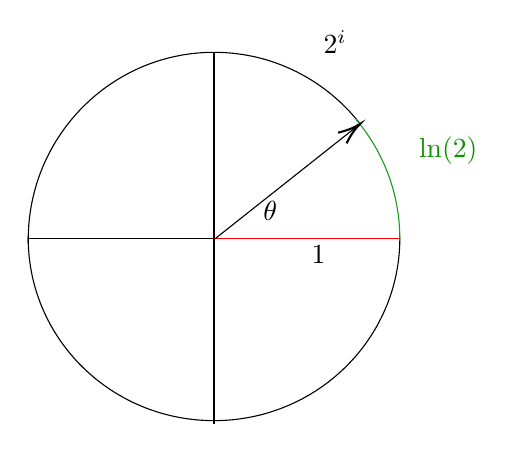
\begin{tikzpicture}[x=0.75pt,y=0.75pt,yscale=-1,xscale=1]
%uncomment if require: \path (0,300); %set diagram left start at 0, and has height of 300

%Straight Lines [id:da5300201460555855] 
\draw    (100,164.5) -- (189.5,164.5) ;
%Straight Lines [id:da7209499549539827] 
\draw    (189.5,254) -- (189.5,75) ;
%Shape: Arc [id:dp1477018513826992] 
\draw  [draw opacity=0] (100,167.2) .. controls (99.99,166.57) and (99.98,165.94) .. (99.98,165.31) .. controls (99.98,115.43) and (140.06,75) .. (189.51,75) .. controls (218.06,75) and (243.49,88.49) .. (259.88,109.49) -- (189.51,165.31) -- cycle ; \draw  [color={rgb, 255:red, 0; green, 0; blue, 0 }  ,draw opacity=1 ] (100,167.2) .. controls (99.99,166.57) and (99.98,165.94) .. (99.98,165.31) .. controls (99.98,115.43) and (140.06,75) .. (189.51,75) .. controls (218.06,75) and (243.49,88.49) .. (259.88,109.49) ;
%Straight Lines [id:da8647831039135583] 
\draw [color={rgb, 255:red, 255; green, 0; blue, 0 }  ,draw opacity=1 ]   (189.5,164.5) -- (279.02,164.5) ;
%Shape: Arc [id:dp5268217987140125] 
\draw  [draw opacity=0] (279.01,164.2) .. controls (279.01,164.3) and (279.02,164.4) .. (279.02,164.5) .. controls (279.02,213.08) and (238.94,252.46) .. (189.5,252.46) .. controls (140.06,252.46) and (99.98,213.08) .. (99.98,164.5) .. controls (99.98,164.29) and (99.99,164.08) .. (99.99,163.88) -- (189.5,164.5) -- cycle ; \draw   (279.01,164.2) .. controls (279.01,164.3) and (279.02,164.4) .. (279.02,164.5) .. controls (279.02,213.08) and (238.94,252.46) .. (189.5,252.46) .. controls (140.06,252.46) and (99.98,213.08) .. (99.98,164.5) .. controls (99.98,164.29) and (99.99,164.08) .. (99.99,163.88) ;
%Shape: Arc [id:dp1302089202448049] 
\draw  [draw opacity=0] (257.91,107.34) .. controls (271.09,122.89) and (279.03,143.02) .. (279.01,164.98) -- (189.91,164.9) -- cycle ; \draw  [color={rgb, 255:red, 22; green, 156; blue, 30 }  ,draw opacity=1 ] (257.91,107.34) .. controls (271.09,122.89) and (279.03,143.02) .. (279.01,164.98) ;
%Straight Lines [id:da04674799293912846] 
\draw    (189.91,164.9) -- (258.31,110.73) ;
\draw [shift={(259.88,109.49)}, rotate = 501.62] [color={rgb, 255:red, 0; green, 0; blue, 0 }  ][line width=0.75]    (10.93,-3.29) .. controls (6.95,-1.4) and (3.31,-0.3) .. (0,0) .. controls (3.31,0.3) and (6.95,1.4) .. (10.93,3.29)   ;

% Text Node
\draw (235.25,166.9) node [anchor=north west][inner sep=0.75pt]    {$1$};
% Text Node
\draw (287,114.4) node [anchor=north west][inner sep=0.75pt]  [color={rgb, 255:red, 12; green, 148; blue, 0 }  ,opacity=1 ]  {$\ln( 2)$};
% Text Node
\draw (241,63.4) node [anchor=north west][inner sep=0.75pt]    {$2^{i}$};
% Text Node
\draw (212,145.4) node [anchor=north west][inner sep=0.75pt]    {$\theta $};


\end{tikzpicture}

\subsubsection{Law of Cosines}

Triangles can be characterized by vectors as such, \( \vb{a} + \vb{b} + \vb{c} = 0 \).

\noindent
\begin{tikzpicture}[x=0.75pt,y=0.75pt,yscale=-1,xscale=1]
%uncomment if require: \path (0,300); %set diagram left start at 0, and has height of 300

%Curve Lines [id:da4423317108802115] 
\draw [color={rgb, 255:red, 255; green, 0; blue, 0 }  ,draw opacity=1 ]   (77.15,205.12) .. controls (201.44,203.62) and (289.8,139.23) .. (295.79,37.4) ;
%Straight Lines [id:da9534342452823479] 
\draw    (75.65,247.05) -- (297.28,247.05) ;
%Straight Lines [id:da33389606852560494] 
\draw    (75.65,35.9) -- (75.65,247.05) ;
%Shape: Circle [id:dp26393026690295507] 
\draw   (163,192) .. controls (163,190.9) and (163.9,190) .. (165,190) .. controls (166.1,190) and (167,190.9) .. (167,192) .. controls (167,193.1) and (166.1,194) .. (165,194) .. controls (163.9,194) and (163,193.1) .. (163,192) -- cycle ;
%Shape: Circle [id:dp10820914245059055] 
\draw   (123,201) .. controls (123,199.9) and (123.9,199) .. (125,199) .. controls (126.1,199) and (127,199.9) .. (127,201) .. controls (127,202.1) and (126.1,203) .. (125,203) .. controls (123.9,203) and (123,202.1) .. (123,201) -- cycle ;
%Shape: Circle [id:dp5803203757563192] 
\draw   (202,176) .. controls (202,174.9) and (202.9,174) .. (204,174) .. controls (205.1,174) and (206,174.9) .. (206,176) .. controls (206,177.1) and (205.1,178) .. (204,178) .. controls (202.9,178) and (202,177.1) .. (202,176) -- cycle ;
%Shape: Circle [id:dp5182181490141611] 
\draw   (255,137) .. controls (255,135.9) and (255.9,135) .. (257,135) .. controls (258.1,135) and (259,135.9) .. (259,137) .. controls (259,138.1) and (258.1,139) .. (257,139) .. controls (255.9,139) and (255,138.1) .. (255,137) -- cycle ;

% Text Node
\draw (71.9,262.4) node [anchor=north west][inner sep=0.75pt]    {$0$};
% Text Node
\draw (45,196.4) node [anchor=north west][inner sep=0.75pt]    {$1$};
% Text Node
\draw (167,193.4) node [anchor=north west][inner sep=0.75pt]  [color={rgb, 255:red, 255; green, 0; blue, 4 }  ,opacity=1 ]  {$e$};
% Text Node
\draw (163,263.4) node [anchor=north west][inner sep=0.75pt]    {$1$};
% Text Node
\draw (150,55.4) node [anchor=north west][inner sep=0.75pt]    {$e^{t}$};
% Text Node
\draw (127,202.4) node [anchor=north west][inner sep=0.75pt]    {$a$};
% Text Node
\draw (208,179.4) node [anchor=north west][inner sep=0.75pt]    {$b$};
% Text Node
\draw (261,140.4) node [anchor=north west][inner sep=0.75pt]    {$c$};


\end{tikzpicture}

Then \( \vb{c} = -(\vb{a} + \vb{b}) \).
Thus
\begin{align*}
\norm{\vb{c}}^2 &= (\vb{a} + \vb{b}) \vdot (\vb{a} + \vb{b}) =
(a_1 e_1 + a_2 e_2) \vdot (b_1 e_1 + b_2 e_2) \\
&= \norm{\vb{a}}^2 + \norm{\vb{b}}^2 + \norm{\vb{a}} \norm{\vb{b}} \cos(\theta) \\
&= \norm{\vb{a}}^2 + \norm{\vb{b}}^2 - \norm{\vb{a}} \norm{\vb{b}} \cos(\theta_i).
\end{align*}

\subsubsection{Cauchy-Schwartz Inequality}

This inequality says that \( \abs{\vb{u} \vdot \vb{v}} \leq \norm{\vb{u}} \norm{\vb{v}} \).
This is because
\( \frac{\vb{u} \vdot \vb{v}}{\norm{\vb{u}} \norm{\vb{v}}} = \cos(\theta) \)
thus
\begin{align*}
-1 \leq \frac{\vb{u} \vdot \vb{v}}{\norm{\vb{u}} \norm{\vb{v}}} \leq 1 \implies
\abs{\vb{u} \vdot \vb{v}} \leq \norm{\vb{u}} \norm{\vb{v}}.
\end{align*}
This is just the triangle inequality on the orthogonal decomposition.
Let \( \vb{p} = P_{\vb{u}}(\vb{v}) \).
Then \( \vb{v} = \vb{p} + (\vb{v} - \vb{p}) \)

\noindent
\begin{tikzpicture}[x=0.75pt,y=0.75pt,yscale=-1,xscale=1]
%uncomment if require: \path (0,300); %set diagram left start at 0, and has height of 300

%Straight Lines [id:da34800919926202234] 
\draw [color={rgb, 255:red, 0; green, 0; blue, 0 }  ,draw opacity=1 ]   (99.75,227.18) -- (330.71,112.81) ;
\draw [shift={(332.5,111.93)}, rotate = 513.6600000000001] [color={rgb, 255:red, 0; green, 0; blue, 0 }  ,draw opacity=1 ][line width=0.75]    (10.93,-3.29) .. controls (6.95,-1.4) and (3.31,-0.3) .. (0,0) .. controls (3.31,0.3) and (6.95,1.4) .. (10.93,3.29)   ;
%Straight Lines [id:da63748929084913] 
\draw [color={rgb, 255:red, 255; green, 0; blue, 0 }  ,draw opacity=1 ]   (99.75,227.18) -- (219.09,168.63) ;
\draw [shift={(220.88,167.75)}, rotate = 513.87] [color={rgb, 255:red, 255; green, 0; blue, 0 }  ,draw opacity=1 ][line width=0.75]    (10.93,-3.29) .. controls (6.95,-1.4) and (3.31,-0.3) .. (0,0) .. controls (3.31,0.3) and (6.95,1.4) .. (10.93,3.29)   ;
%Straight Lines [id:da537720110515903] 
\draw [color={rgb, 255:red, 0; green, 95; blue, 255 }  ,draw opacity=1 ]   (220.88,167.75) -- (164.39,73.1) ;
\draw [shift={(163.36,71.38)}, rotate = 419.16999999999996] [color={rgb, 255:red, 0; green, 95; blue, 255 }  ,draw opacity=1 ][line width=0.75]    (10.93,-3.29) .. controls (6.95,-1.4) and (3.31,-0.3) .. (0,0) .. controls (3.31,0.3) and (6.95,1.4) .. (10.93,3.29)   ;
%Straight Lines [id:da16959396821644424] 
\draw    (99.75,227.18) -- (162.61,73.23) ;
\draw [shift={(163.36,71.38)}, rotate = 472.21] [color={rgb, 255:red, 0; green, 0; blue, 0 }  ][line width=0.75]    (10.93,-3.29) .. controls (6.95,-1.4) and (3.31,-0.3) .. (0,0) .. controls (3.31,0.3) and (6.95,1.4) .. (10.93,3.29)   ;
%Straight Lines [id:da8403058073952824] 
\draw    (99.75,227.18) -- (162.61,73.23) ;
\draw [shift={(163.36,71.38)}, rotate = 472.21] [color={rgb, 255:red, 0; green, 0; blue, 0 }  ][line width=0.75]    (10.93,-3.29) .. controls (6.95,-1.4) and (3.31,-0.3) .. (0,0) .. controls (3.31,0.3) and (6.95,1.4) .. (10.93,3.29)   ;

% Text Node
\draw (222.83,178.77) node [anchor=north west][inner sep=0.75pt]  [color={rgb, 255:red, 255; green, 0; blue, 0 }  ,opacity=1 ]  {$p=P_{u}( v)$};
% Text Node
\draw (202.31,100.35) node [anchor=north west][inner sep=0.75pt]  [color={rgb, 255:red, 0; green, 104; blue, 255 }  ,opacity=1 ]  {$v -p$};
% Text Node
\draw (149.98,43.4) node [anchor=north west][inner sep=0.75pt]    {$v$};
% Text Node
\draw (341.98,110.4) node [anchor=north west][inner sep=0.75pt]    {$u$};


\end{tikzpicture}



\subsection{Outer Product}

The outer product between two vectors \( \vb{u} \wedge \vb{v} \)
is an oriented area.



\end{document}